\section{Evaluation}

The multi-label DNN classifier is trained and tested with randomly selected samples by using automated script which splits the dataset with 80\% for training and 20\% for test. We train the model 100 steps with training samples. For each training step, the training sample is shuffled randomly to protect the model learns biased due to the order of training samples.

\begin{figure}[t]
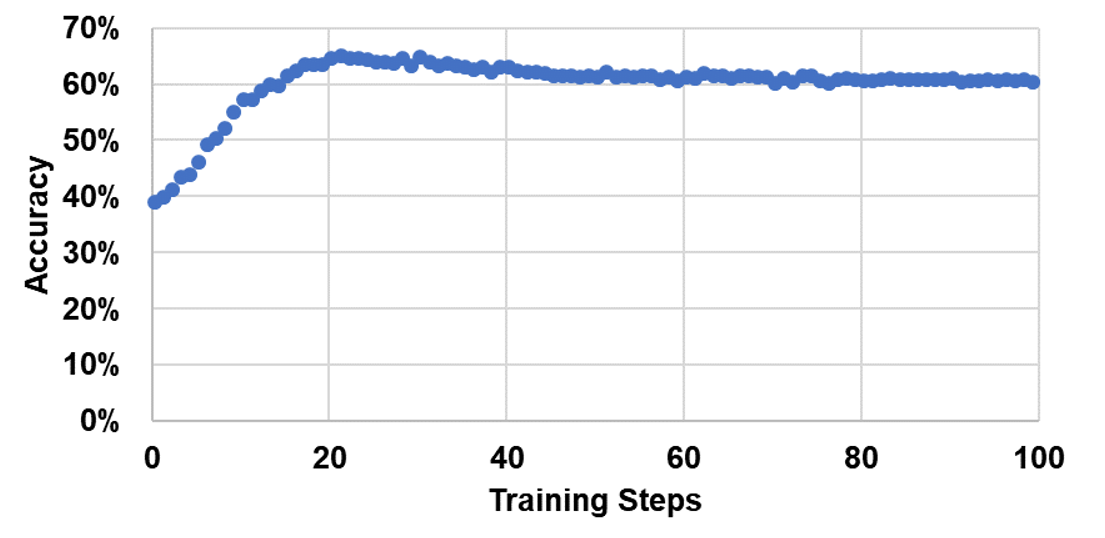
\includegraphics[width=0.48\textwidth]{figs/accuracy_dnn_model.png}
\caption{Overall accuracy with multiple training steps}
\label{fig:accuracy_dnn_model}
\end{figure}

Figure~\ref{fig:accuracy_dnn_model} shows the overall accuracy of the classifier while training the model multiple steps. The maximum accuracy is 65.4\% when the training step is 22. The accuracy increases when the step is less than 22, because the model is underfitted. After trains more than 22 steps, accuracy decreases, because of overfitting.

\begin{figure}[t]
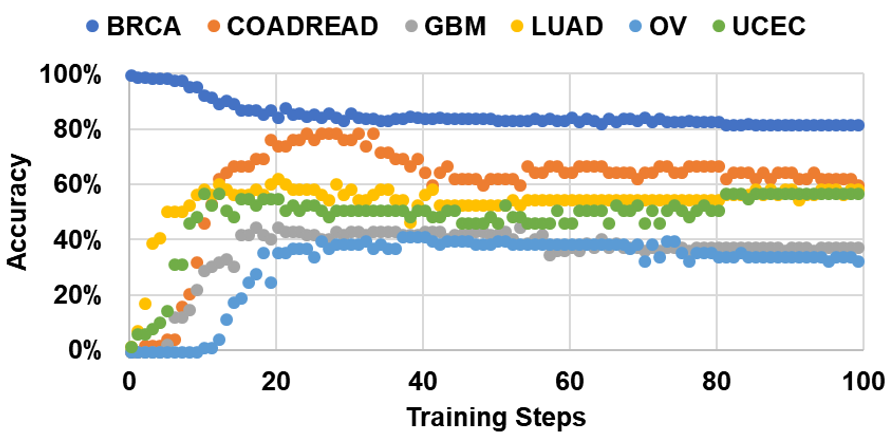
\includegraphics[width=0.48\textwidth]{figs/accuracy_dnn_cancer.png}
\caption{Accuracy for each cancer types}
\label{fig:accuracy_dnn_cancer}
\end{figure}

Figure~\ref{fig:accuracy_dnn_cancer} shows the accuracy of each cancer type while training step increases. When the model is underfitted (i.e., less than 22 training steps), the model predicts cancer type for the sample as BRCA, because it is majority of dataset. Therefore, the accuracy for BRCA is nearly 100\%, but the accuracy of other cancer types are small. As training step increases, the model predicts other cancer types with sacrificing accuracy of BRCA prediction. Whn the model is overfitted (i.e., more than 22 training steps), prediction accuracy for all types are decreasing tendency.
